\subsection{Aufbau von X3D}

Zwei Jahre nach Veröffentlichung des VRML97-Standards begann eine Arbeitsgruppe des Web3D Consortiums 1999 mit der Entwicklung des Nachfolgers von VRML, \emph{Extensible 3D} \autocite{Daly:2007}. Dieser X3D abgekürzte, freie Standard wurde 2004 ebenso wie zuvor VRML zu einem ISO-Standard\footnote{ISO/IEC 19775-1.} \autocite{Brutzman:2007:XEG:1214715}. Bei der Entwicklung X3Ds wurde auf eine Abwärtskompatiblität zu VRML97 geachtet. Das \enquote{\emph{X}} im Namen impliziert bereits die Nutzung der \emph{Extensible Markup Language (XML)} als Grundlage dieses neuen Grafikformats. Hierdurch wurde eine größere Konvergenz zu bestehenden Webtechnologien wie HTML und XHTML erzielt.

X3D nutzt einen gerichteten, azyklischen Szenengraph zur Repräsentation einer 3D-Szene (vgl. Abbildung \ref{FIG:SCENEGRAPH_EXAMPLE}). Knoten unterhalb der Wurzel des Graphen (dem \emph{Universum}) stellen dabei sämtliche Objekte der Welt dar. Die X3D-Spezifikation definiert eine große Zahl von Knoten, welche alle benötigten Elemente einer Grafikdarstellung wie Geometrien, Lichtquellen, Kameras, Texturen, Transformationen et cetera abbilden. Der Szenengraph kann in drei Formaten abgespeichert werden. Zur Verfügung stehen ein XML-Format, die klassische VRML-Notation und schließlich ein komprimiertes Binärformat \autocite{Daly:2007}. Für die Darstellung des Formats ist ein spezieller \emph{X3D-Viewer} notwendig. Dieser erzeugt aus dem X3D-Szenengraph eine 3D-Darstellung, die frei von allen Seiten betrachtet werden kann.

Da die X3D-Spezifikation sehr umfangreich ist, existieren sogenannte \emph{Profile}, welche eine Menge von Knoten für eine bestimmte Anwendungsdomäne bündeln. Hierdurch ist es möglich, nur tatsächlich benötigte Knoten des Standards zu laden.

\subsection{Das Framework X3DOM}

\subsubsection{Entstehung}

Während der Ausarbeitung des neuen HTML5-Standards stellte X3D den vom World Wide Web Consortium favorisierten Standard für die Realisierung von Web3D-Inhalten dar. Der Arbeitsentwurf der HTML5-Spezifikationen aus dem Jahr 2009 vermerkt diesbezüglich:

\begin{itquote}
	\enquote{Embedding 3D imagery into XHTML documents is the domain of X3D, or technologies based on X3D that are namespace-aware.} \autocite{W3C_HTML5_SPEC_WORKING_DRAFT_12_2009}
\end{itquote}

Diese äußerst knappe Formulierung definiert jedoch in keinster Weise näher, wie eine Plugin-freie Integration von X3D in HTML aussehen könnte. Behr et al. vom Fraunhofer Institut für graphische Datenverarbeitung Darmstadt publizierten daraufhin im selben Jahr ihren Ansatz, wie X3D-Inhalte direkt in HTML eingebettet werden könnten \autocite{Behr:2009:XDH:1559764.1559784}. Ziel des vorgeschlagenen Integrations-Modells \emph{X3DOM} ist eine wechselseitige Verknüpfung zwischen bestehenden Webtechnologien wie dem \emph{Document Object Model} und X3D. Die Autoren erhoffen sich, langfristig eine ähnliche Entwicklung anzustoßen, wie sie das Vektorgrafikformat \emph{Scalable Vector Graphics} (SVG) im WWW durchlief \autocite{Behr:2009:XDH:1559764.1559784}. Während SVG zunächst nur in einigen wenigen Browsern unterstützt wurde, ist dieser Standard inzwischen überall nativ implementiert \autocite{CANIUSE_SVG}. Zum Zeitpunkt der Veröffentlichung dieser Arbeit lag X3DOM noch in einer frühen \emph{Pre-Alpha}-Version vor und zahlreiche Details der Implementierung blieben offen.

\subsubsection{Architektur}
\label{SEC:X3D_ARCHITECTURE}

Im darauffolgenden Jahr legten \textcite{Behr:2010:SAH:1836049.1836077} in einer weiteren Arbeit die zuvor abstrakt dargestellten Ideen ihres Modells mittels der inzwischen gereiften Architektur des X3DOM-Frameworks konkret dar. Grundgedanke von X3DOM ist die Bereitstellung einer einheitlichen Schnittstelle zur deklarativen Programmierung von 3D-Szenen. Hierbei werden die direkt innerhalb des HTML-Dokuments eingebetteten X3D-Knoten wechselseitig mit dem X3D-System synchronisiert. Durch das Hinzufügen, Löschen und Abändern dieser DOM-Elemente kann der Anwendungs-Entwickler die 3D-Szene mittels einfacher JavaScript-Aufrufe dynamisch anpassen.
Zusätzlich zu den im X3D-Standard spezifizierten Attributen fügt X3DOM vielen Knoten weitere Eigenschaften hinzu, die deren Benutzung weiter vereinfachen.

\begin{figure}
	\centering
	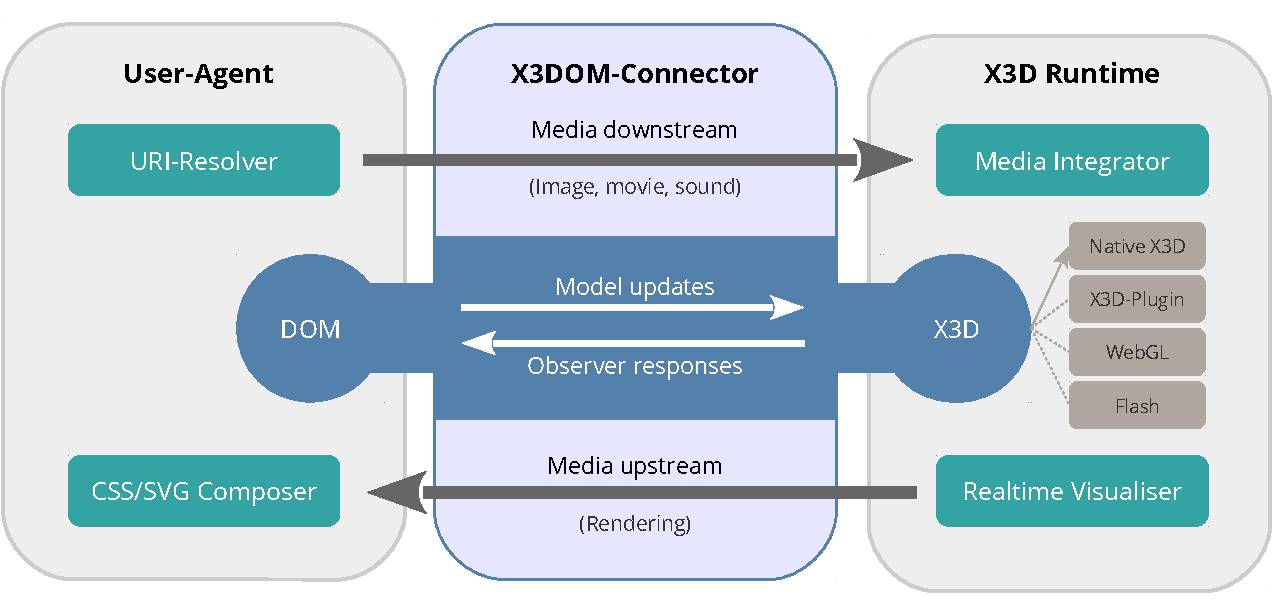
\includegraphics[width=0.9\textwidth]{kap4/x3d/figures/x3dom_architecture-crop.pdf}
	\caption{Architektonischer Aufbau von X3DOM. Geringfügig adaptiert nach \textcite{Behr:2010:SAH:1836049.1836077}.}
	\label{FIG:X3DOM_ARCHITECTURE}
\end{figure}

Die in Abbildung \ref{FIG:X3DOM_ARCHITECTURE} gezeigte Architektur X3DOMs besteht im Wesentlichen aus drei Komponenten: Dem \emph{User Agent}, dem X3DOM-Connector und dem X3D-Runtime.

Ersteres entspricht hier dem Webbrowser. Dieser enthält das Document Object Model und die hierin integrierten X3D-Knoten. Der Browser ermöglicht es weiterhin Multimedia-Dateien wie Grafiken, Video und Audio durch seinen \emph{URI-Resolver} von einem Server herunterzuladen, um diese X3D bereit zu stellen.

Das X3D-Runtime-Objekt auf der andern Seite des Schemas ist für das eigentliche Rendering der Szene und die Verarbeitung von Benutzereingaben verantwortlich. Die Architektur erlaubt hierbei mehrere sogenannter \emph{Backends}. Ein Backend stellt die Technologie dar, mit welcher die computergrafischen Berechnungen vollzogen werden. Mittels eines Fallback-Systems wird das Rendering-Backend anhand einer Priorisierung der Technologien ausgewählt. Hierbei wird zunächst überprüft, ob der der Webbrowser X3D nativ darstellen kann oder ob alternativ ein X3D-Plugin vorhanden ist. Schlägt dies fehl, so wird das Rendering durch WebGL realisiert. Ist auch diese Technik nicht verfügbar, wird auf das proprietäre Flash-Plugin ausgewichen. Wenn dies ebenfalls scheitert, kann keine 3D-Darstellung erfolgen \autocite{Behr:2010:SAH:1836049.1836077}. Die X3D-Runtime-Komponente beinhaltet weiterhin einen sogenannten \emph{Media Integrator}, der die vom User Agent geladenen Medien wie beispielsweise Texturen verarbeitet.

Der \emph{X3DOM Connector} fungiert schließlich als Mittelsmann der zwei obigen Komponenten. Er stellt die Verbindung zwischen den X3D-Knoten im DOM des HTML-Dokuments und dem X3D-System her und synchronisiert diese. Wird das DOM durch JavaScript manipuliert, so wird dies an das Runtime-Objekt propagiert, welches die Szene entsprechend neu rendert und das Bild durch den \emph{Media Upstream} an das HTML-Dokument weiterleitet. Gleichzeitig reagiert das System durch ein \emph{Observer}-Entwurfsmuster auf Benutzereingaben, welche durch JavaScript-Events wie \emph{onClick} abgebildet werden.

\subsection{Beispiel: Rotierende Pyramide}
\label{SEC:X3D_EXAMPLE}

Anhand eines einfachen Beispiels wird im Folgenden der strukturelle Aufbau und einige grundlegenden Konzepte einer X3DOM-basierten Grafikdarstellung aufgezeigt, indem der Quelltext konkret Schritt für Schritt erläutert werden. Das Beispiel und sein Gegenstück in WebGL ist auf der beigefügten CD enthalten.

Die exemplarische Anwendung stellt eine Pyramide dar, welche um die Y-Achse rotiert. Durch eine Auswahlliste kann aus einer perspektivischen oder einer orthogonalen Parallelenprojektion gewählt werden. Abbildung \ref{FIG:X3DOM_EXAMPLE_PROJECTIONS} zeigt diese zwei verschiedenen Ansichten. Die Rotation der Figur kann zudem mittels eines Kontrollkästchens (\emph{Checkbox}) jederzeit pausiert werden.

\begin{figure}[htb]
	\centering
	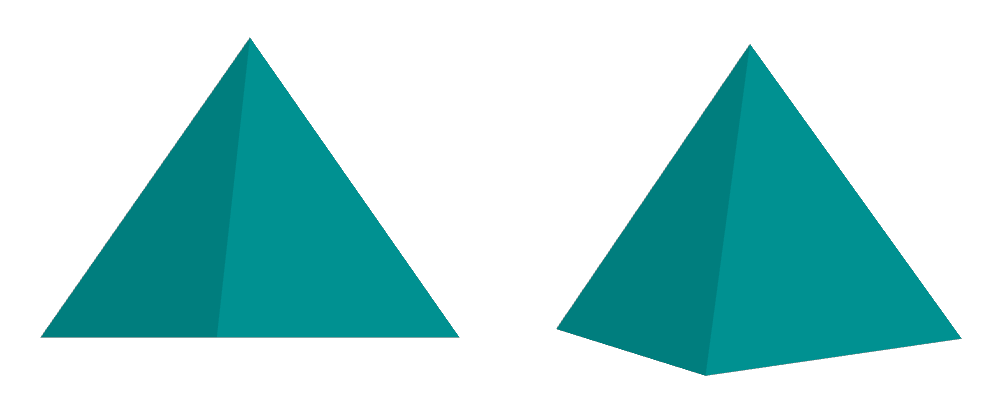
\includegraphics[width=0.6\textwidth]{kap4/x3d/figures/example_orthogonal_vs_perspective.png}
	\caption{Orthogonale und perspektivischen Darstellung der Pyramide.}
	\label{FIG:X3DOM_EXAMPLE_PROJECTIONS}
\end{figure}

Eine große Stärke X3Ds im Hinblick auf die Nutzung im Word Wide Web liegt in der großen Nähe zu HTML. Da beide Sprachen Anwendungen der Standard Generalized Markup Language (SGML) sind, ist ihr syntaktischer Aufbau sehr ähnlich. Schlüsselworte in eckigen Klammern, sogenannte \enquote{\emph{Tags}}, dienen der logischen und hierarchischen Strukturierung der Inhalte. Ein Knoten kann zusätzlich durch verschiedene Attribute parametrisiert werden.

\smallskip
\begin{listing}[!h]
\begin{htmlcode}
<head>
	<script src='x3dom.js'></script>
</head>
<body>
	<h1>Konventioneller HTML-Code</h1>
	<X3D width='800px' height='600px'>
		<Scene>
			<!-- Elemente des Szenengraphs -->
		</Scene>
	<X3D>
</body>
\end{htmlcode}
\caption{Einbettung des X3D-Szenengraphs in HTML}
\label{LISTING:X3D_EXAMPLE_EMBEDDING_SCENEGRAPH}
\end{listing}

Nach dem Laden des X3DOM-Quelltexts im Kopfbereich eines HTML-Dokuments kann X3D direkt in dieses eingebunden werden. Listing \ref{LISTING:X3D_EXAMPLE_EMBEDDING_SCENEGRAPH} zeigt diese Einbettung mittels des speziellen X3D-Tags. Durch Angabe der \textit{width}- und \textit{height}-Attribute wird die benötigte Größe der Zeichenfläche spezifiziert. Dem X3D-Tag direkt untergeordnet liegt die Wurzel des Szenengraphen, welche sämtlichen weiteren Knoten der Anwendung enthält. Um die Lesbarkeit der folgenden Ausführungen zu gewährleisten, wurde der komplette Quelltext der Szene in Listing \ref{LISTING:X3D_EXAMPLE} auf der nächsten Seite abgedruckt.

\smallskip
\begin{listing}[p]
\htmlinput[firstline=19, lastline=60, firstnumber=19]{kap4/x3d/example/index.html}
\caption{Gesamter Szenengraph des Beispiels.}
\label{LISTING:X3D_EXAMPLE}
\end{listing}

Das kleine Programm kann im Wesentlichen in drei Schritte gegliedert werden:

\smallskip
\begin{enumerate}[noitemsep]
	\item Festlegen der Ansicht und des Navigationsmodus.
	\item Erstellung und Transformation der Pyramiden-Geometrie.
	\item Animation der Figur.
\end{enumerate}

Zunächst wird die Ansicht der Szene mittels des \textit{Viewpoint}-Elements in den Zeilen 21 bis 23 festgelegt. Der Darstellung können beliebig viele solcher Viewpoints hinzugefügt werden. Durch JavaScript können diese anschließend angesteuert und dynamisch aktiviert werden.
Standardmäßig wird hierbei eine perspektivische Projektion verwendet. Für eine orthogonale Parallelenprojektion steht der \textit{OrthoViewpoint} zur Verfügung.
Das \textit{NavigationInfo}-Element definiert daraufhin das Navigationsmodell der Szene, also die Art und Weise, wie die Darstellung durch den Benutzer interaktiv verändert werden kann. X3DOM bietet hierbei eine Vielzahl verschiedener vorgefertiger Modi \autocite{X3DOM_DOCS_NAVIGATION_INFO_NODE}: Während die Kamera bei manchen Modelle frei bewegt werden kann, sind andere auf die nähere Betrachtung eines einzelnen Objekts zugeschnitten. Im Beispiel ist eine solche Navigation deaktiviert.

3D-Modelle werden in X3D mittels des \textit{Shape}\footnote{Engl. für Form oder Gestalt.}-Knotens umgesetzt. Das Format bietet für zahlreiche geometrische Primitive wie Kugeln, Quader, Zylinder et cetera bereits vordefinierte Elemente, die die Erstellung dieser Basisfiguren sehr einfach gestalten. Listing \ref{LISTING:X3D_SHAPE_NODE} zeigt dies exemplarisch durch Deklaration eines Würfels mittels des \textit{Box}-Tags in Zeile 5. Dem Shape-Knoten ist weiterhin das \textit{Appearance}-Element untergeordnet, welches wiederum einen \textit{Material}-Knoten enthält (vgl. Listing \ref{LISTING:X3D_EXAMPLE}, Zeilen 43 - 45). Dieser legt zahlreiche Attribute hinsichtlich der Beleuchtung des Objekts fest: etwa die Reflexionsintensität des ambienten Lichts, die Farbe diffusen Lichts, den Grad spekularer Glanzeffekte und so weiter fest.

\smallskip
\begin{listing}[!h]
\begin{htmlcode}
<Shape>
	<Appearance>
		<Material diffuseColor='0 0.66 0.66'></Material>
	</Appearance>
	<Box></Box>
</Shape>
\end{htmlcode}
\caption{Erstellung einfacher Primitive durch den Shape-Knoten.}
\label{LISTING:X3D_SHAPE_NODE}
\end{listing}

Sofern das Modell durch kein geometrisches Primitiv dargestellt werden kann, bietet X3D durch das \textit{IndexedFaceSet}-Element einen Mechanismus, wie die topologische Struktur eines 3D-Modells durch explizite Angabe der Vertices und Seiten definiert werden kann. Unter der Topologie wird in diesem Zusammenhang die Nachbarschaftsbeziehung der Knotenpunkte, Kanten und Flächenstücke einer Geometrie verstanden. Der IndexedFaceSet-Knoten befindet sich unmittelbar unterhalb des Shape-Elements.
Die Seiten der Figur werden dabei mittels des \textit{CoordIndex}-Elements spezifziert. Durch Angabe dreier oder mehr Indices, der im Kindknoten \textit{Coordinate} gegebenen Vertices, wird ein entsprechendes Polygon erstellt (Zeile 28 ff.). Die Zahl $-1$ dient dabei als Begrenzungszeichen der verschiedenen Seiten. Zu beachten gilt zudem, dass die Indexierung der Vertices bei $0$ beginnt.
Der so kreierten Pyramide wird mittels des \textit{diffuseColor}-Attributs des Material-Knotens die Farbe Türkis zugeordnet (Zeile 44). Farben werden in X3D durch das RGB-Farbmodell angegeben, wobei $1$ der maximalen Intensität eines Farbkanals entspricht.

Die gesamte Geometrie wird durch ein Transformations-Element umhüllt. Dieses ermöglicht die affine Transformation untergeordneter Elemente. In diesem Fall wird die Pyramide in die negative Y-Richtung translatiert (Zeile 26). Das Attribut \textit{DEF} dient der eindeutigen Bezeichnung des Knotens und wird im finalen Animations-Schritt benötigt.

Animationen werden in X3D durch sogenannte Schlüsselbilder (\emph{Keyframes}) realisiert. Hierbei werden verschiedene diskrete Zustände der Animation durch die Keyframes definiert und die Bewegung anschließend durch lineare Interpolation zwischen diesen Werten erzielt. Innerhalb X3Ds sind hierfür mehrere Komponenten nötig: Zunächst wird ein sogenannter \textit{TimeSensor} definiert, welcher die Interpolation der Werte anstößt und die Länge der Animation durch das Attribut \textit{cycleInterval} festlegt (Zeile 49). Die Schlüsselbilder werden innerhalb eines \textit{Interpolator}-Knotens spezifiziert (Zeile 50 f.). Da die Rotation der Figur verändert werden soll, wird ein \textit{OrientationInterpolator} benötigt. Um eine vollständige Drehung umzusetzen wird das Bogenmaß des Winkel im Intervall von $0$ bis $\pi$ interpoliert.
Um diese zwei Komponenten nun zu verknüpfen, führt X3DOM das Konzept von \textit{Routes} ein. Durch dieses Pipeline-artige Konstrukt kann ein automatischer Datenaustausch zwischen verschiedenen Knoten angestoßen werden, sofern eine bestimmte Bedingung zutrifft (vgl. Zeile 55 ff.). Der Zeitsensor im Beispiel initiiert in regelmäßigen Abständen eine zeitabhängige Neuberechnung des aktuellen Rotationswinkels im \textit{OrientationInterpolator}. Sobald sich der Rotationswinkel entsprechend verändert hat, wird dies an den Transformationsknoten propagiert, welcher nun die Rotation der Pyramide anpasst.

Bei Betrachtung des gesamten Quelltexts des Beispiels in Listing \ref{LISTING:X3D_EXAMPLE} wird die Kompaktheit X3Ds deutlich. Bereits wenige XML-Knoten waren ausreichend, um die gewünschte rotierende Pyramide im Webbrowser darzustellen. Sofern eine manuelle Definition der Geometrie nicht notwendig gewesen wäre, wäre das Programm sogar noch deutlich kürzer ausgefallen. Dies unterstreicht die Vorteile des deklarativen Ansatzes von X3D.

Die eingangs zitierte Nennung X3Ds in der HTML5-Spezifikation ist inzwischen nicht mehr in der aktuellen Revision des Arbeitsentwurfs zu finden. Somit muss X3D nicht mehr zwingend als der offizielle, durch das W3C angestrebte Standard für Web3D betrachtet werden. Mit der Web Graphics Library ist eine starke Alternative für einen solchen offiziell unterstützen Grafikstandards entstanden. Im Folgenden soll dieser näher beleuchtet werden.
